\documentclass{article}

\usepackage{graphicx}
\usepackage{tikz}
\usepackage{tikzsymbols}
\usetikzlibrary{calc,patterns,shapes.geometric}
\pagestyle{empty}
\usepackage[margin=0pt]{geometry}
\geometry{papersize={14in,12in}}

\def\centerarc[#1](#2)(#3:#4:#5){\draw[#1] ($(#2)+({#5*cos(#3)},{#5*sin(#3)})$) arc (#3:#4:#5);}

\begin{document}
	\begin{figure}
		\centering
		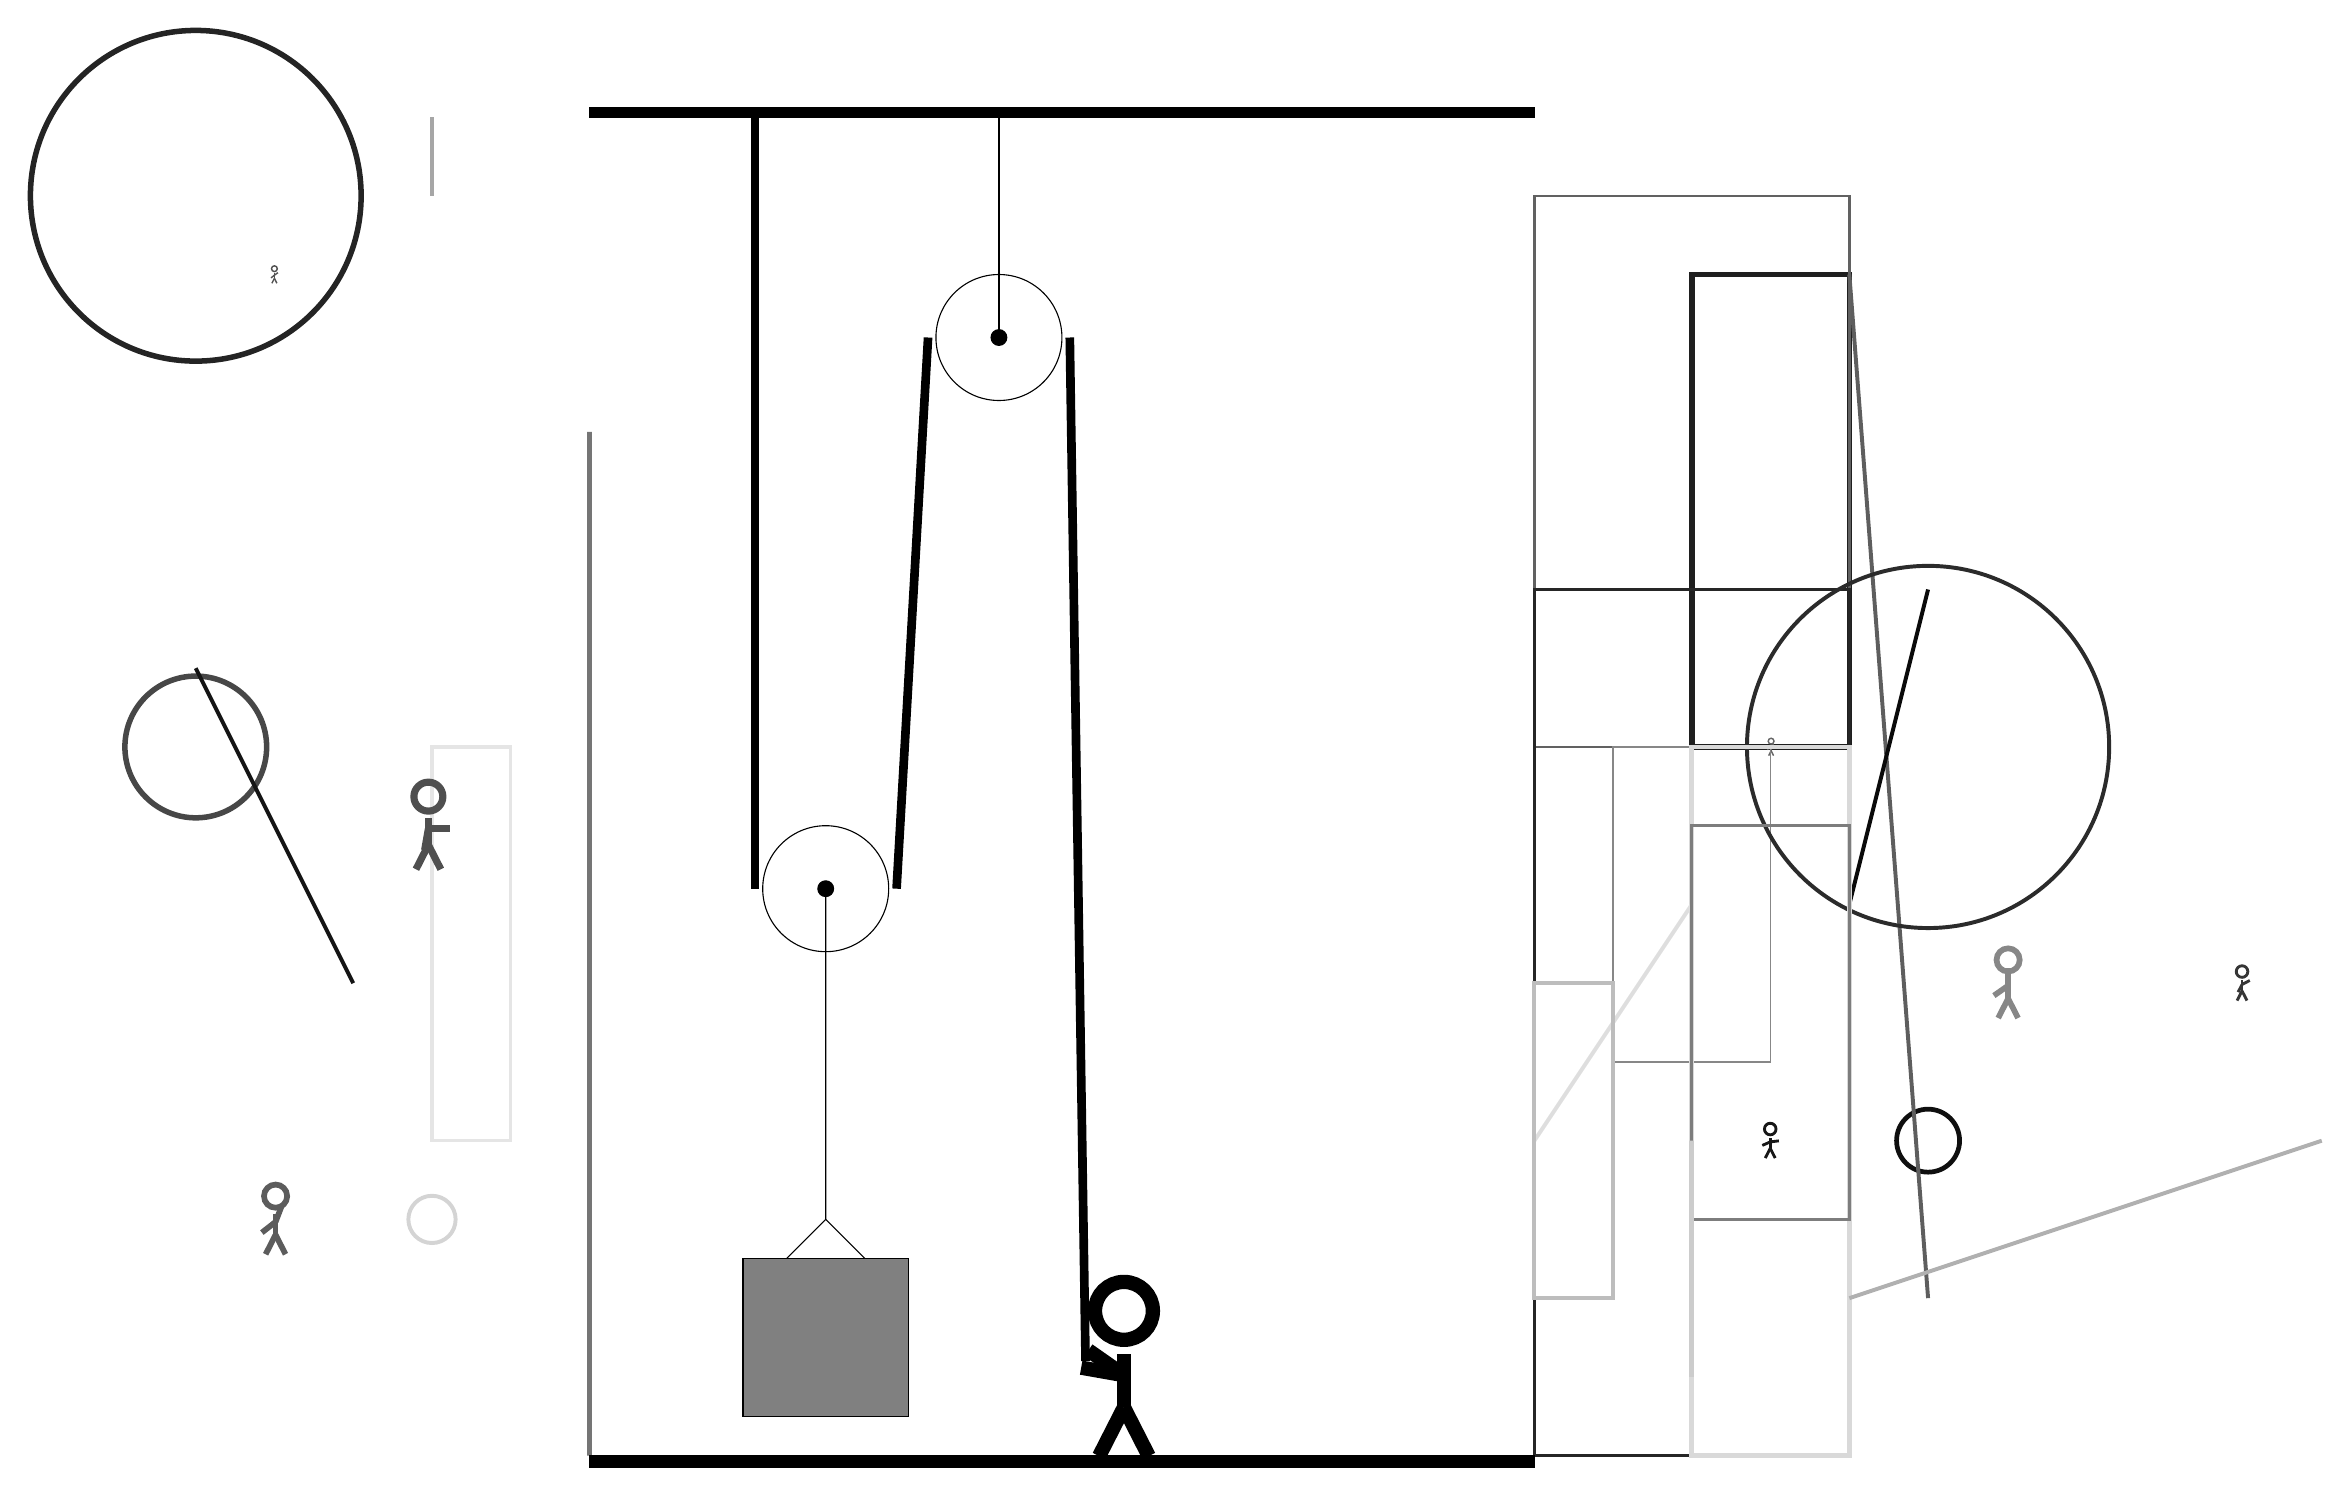
\begin{tikzpicture}
			%%%%% START %%%%%
			
			\draw[fill=black] (-2, 14) rectangle (10, 14.125);
			
			\draw (3.2, 11.2) circle (0.8);
			\draw[fill=black] (3.2, 11.2) circle (0.1);
			\draw[thick] (3.2, 11.2) -- (3.2, 14);
			
			\draw (1, 4.2) circle (0.8);
			\draw[fill=black] (1, 4.2) circle (0.1);
			
			\draw (1, 4.2) -- (1, 0) -- (0.5, -0.5);
			\draw (1, 0) -- (1.5, -0.5);
			\draw[fill=black!50] (-0.05, -0.5) rectangle (2.05, -2.5);
			
			\draw [line width=0.7mm, color=black!72](-7, 6) circle (0.9);
			
			\draw [line width=0.6mm, color=black!94](15, 1) circle (0.4);
			\draw[line width=0.7mm, color=black!88] (12, 6) rectangle (14, 12);
			\draw[line width=0.5mm, color=black!63](15, -1) -- (14, 12);
			\draw[line width=0.3mm, color=black!62] (10, 13) rectangle (14, 6);
			\node[line width=0.7mm, color=black!60] at (13, 6) {\Strichmaxerl[1][25][59]};
			\draw[line width=0.5mm, color=black!88] (12, 6) rectangle (12, 0);
			\draw[line width=0.2mm, color=black!47] (11, 2) rectangle (13, 6);
			\draw[line width=0.5mm, color=black!92](-7, 7) -- (-5, 3);
			\draw[line width=0.4mm, color=black!85] (10, -3) rectangle (14, 8);
			\draw [line width=0.7mm, color=black!86](-7, 13) circle (2.1);
			\draw [line width=0.5mm, color=black!83](15, 6) circle (2.3);
			\draw[line width=0.5mm, color=black!96](15, 8) -- (14, 4);
			\draw[line width=0.4mm, color=black!10] (-4, 1) rectangle (-3, 6);
			\node[line width=0.2mm, color=black!69] at (-4, 5) {\Strichmaxerl[5][80][0]};
			\draw[line width=0.6mm, color=black!35] (-4, 14) rectangle (-4, 13);
			\draw[line width=0.6mm, color=black!15] (12, 6) rectangle (14, -3);
			
			\draw[line width=0.5mm, color=black!13](12, 4) -- (10, 1);
			\node[line width=0.5mm, color=black!79] at (19, 3) {\Strichmaxerl[2][63][27]};
			\draw[line width=0.7mm, color=black!54] (-2, -3) rectangle (-2, 10);
			\node[line width=0.4mm, color=black!47] at (16, 3) {\Strichmaxerl[4][35][90]};
			
			\draw[line width=0.5mm, color=black!31](14, -1) -- (20, 1);
			\node[line width=0.4mm, color=black!68] at (-6, 12) {\Strichmaxerl[1][40][35]};
			\draw[line width=0.4mm, color=black!51] (12, 5) rectangle (14, 0);
			\draw[line width=0.5mm, color=black!26] (10, 3) rectangle (11, -1);
			
			\node[line width=0.4mm, color=black!64] at (-6, 0) {\Strichmaxerl[4][38][69]};
			\draw [line width=0.4mm, color=black!51](-8, 4) circle (0.0);
			\draw[line width=0.6mm, color=black!20] (12, -2) rectangle (12, 1);
			\draw [line width=0.5mm, color=black!17](-4, 0) circle (0.3);
			\node[line width=0.7mm, color=black!91] at (13, 1) {\Strichmaxerl[2][24][7]};
			
			\draw[line width=1.1mm] (0.1, 14) -- (0.1, 4.2);
			\centerarc[line width=1.1mm](1, 4.2)(180:360:0.9);
			\draw[line width=1.1mm](1.9, 4.2) -- (2.3, 11.2);
			\centerarc[line width=1.1mm](3.2, 11.2)(0:180:0.9);
			\draw[line width=1.1mm](4.1, 11.2) -- (4.3, -1.8);
			
			\node at (4.7, -1.9) {\Strichmaxerl[10][-35][170]};
			
			\draw[fill=black] (-2, -3) rectangle (10, -3.15);
			
			%%%%% END %%%%%
		\end{tikzpicture}
	\end{figure}	
\end{document}